% Chapter 1

\chapter{Introducción General} % Main chapter title

\label{Chapter1} % For referencing the chapter elsewhere, use \ref{Chapter1} 
\label{IntroGeneral}

%----------------------------------------------------------------------------------------

% Define some commands to keep the formatting separated from the content 
\newcommand{\keyword}[1]{\textbf{#1}}
\newcommand{\tabhead}[1]{\textbf{#1}}
\newcommand{\code}[1]{\texttt{#1}}
\newcommand{\file}[1]{\texttt{\bfseries#1}}
\newcommand{\option}[1]{\texttt{\itshape#1}}
\newcommand{\grados}{$^{\circ}$}

%----------------------------------------------------------------------------------------

\section{ Introducción General }

El presente caso de estudio ocurre en un contexto muy común dado en la producción industria a baja escala: los operarios son los encargados de manipular y operar prácticamente todas las etapas. Cuando surge la necesidad de mejorar la calidad del producto en necesario modernizar parte o el total de esta linea de producción. Como consecuencia los costos de automatizarla de manera integra implican una gran inversión inicial muy grande. Mas aun cuando se trata de hacerlo a través de soluciones armadas llave en mano de empresas normalmente extranjeras.

%----------------------------------------------------------------------------------------
\section{ Lineas de producción asistidas }

La forma mas básica de asistir un proceso industrial es a través de brindarle al operador indicadores del estado del proceso, ya sea en forma de alarmas o señales luminosas. El mismo solo se limita a manipular llaves, pulsadores y atender la interrupción en caso de anomalía. 
En un sistema totalmente automatizado en cambio el operador solo se limitaría a dar inicio al proceso y a atender las alarmas en caso de alguna falla o anomalía.

Las soluciones para este tipo de entornos se logra a partir de un sistema de control distribuido con un modulo principal y varios submódulos, que en la cual el modulo principal es el encargado de tomar la información de los submódulos y ejecuta las acciones correspondientes. 
Otra forma es usar módulos independientes entre si en donde cada uno se encarga de monitorear y controlar parámetros de una determinada etapa.

\section{ Necesidad y motivación }

La necesidad de incrementar los niveles de calidad y el volumen de producción determinaron la decisión de construir una nueva planta mas moderno estandarizada y con sistemas de monitoreo de parámetros críticos del proceso, dejando si en una primera etapa el control en manos del operador.

Adicionalmente era vital tener registro integro de parámetros del proceso y de las acciones ejecutadas por los operadores, a modo de poder verificar y auditar posteriormente el proceso en caso de detectar anomalías en el producto.

Se planteo también implementar que la solución debía ser solo una primera etapa que sirviera de puente entre una etapa posterior de automatización del sistema y el sistema manual casi artesanal actual. En la Figura \ref{fig:planta_actual} se puede ver como es la linea de proceso actual.

\begin{figure}[h]
	\centering
	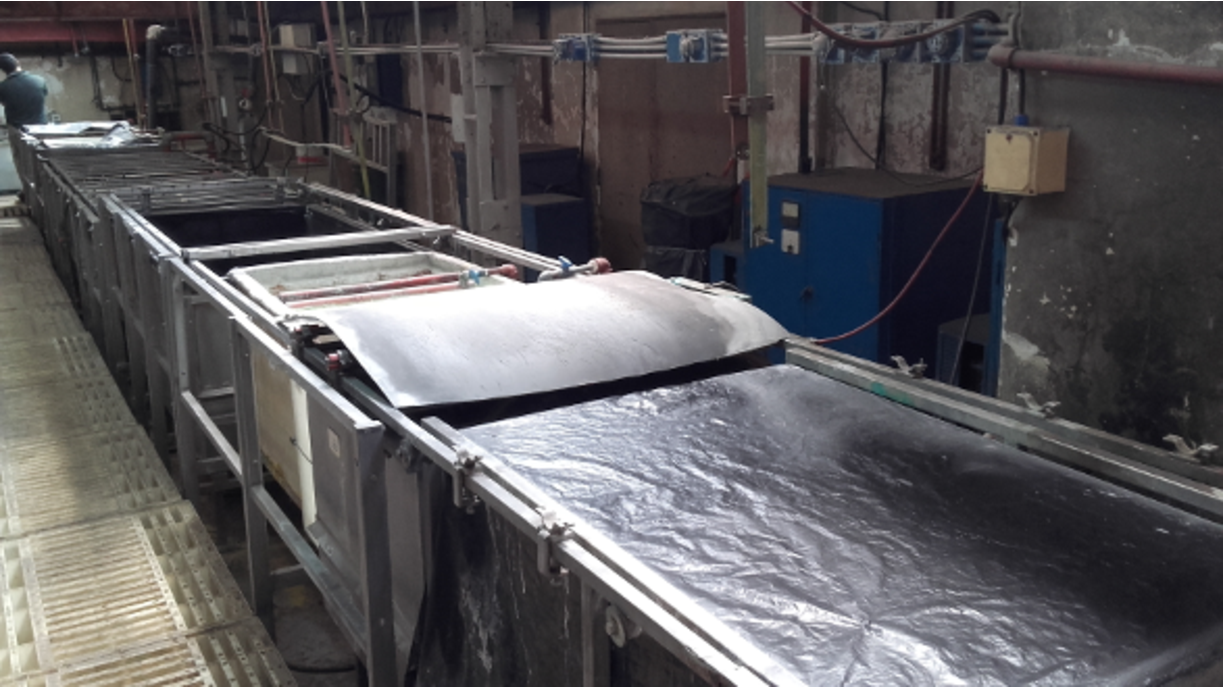
\includegraphics[width=.8\textwidth]{Figures/Cap_1/planta_actual}
	\caption{Linea de galvanizada actual operada manualmente.}
	\label{fig:planta_actual}
\end{figure}

En la Figura \ref{fig:planta_moderna} se puede ver como es una linea de producción totalmente automatizada de otro fabricante.

\begin{figure}[h]
	\centering
	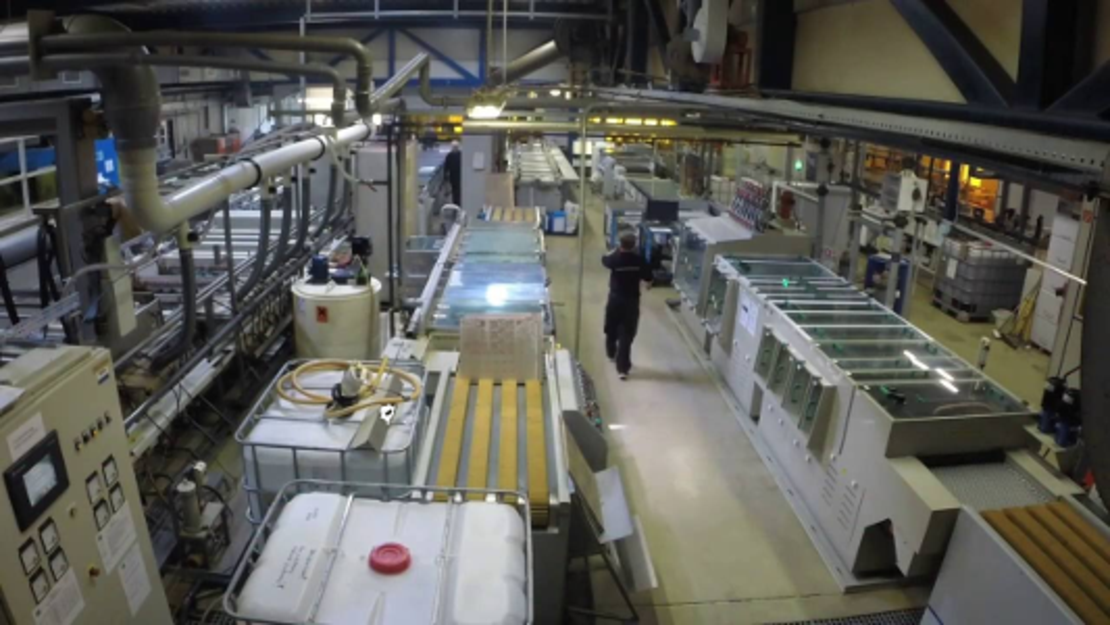
\includegraphics[width=.8\textwidth]{Figures/Cap_1/planta_moderna}
	\caption{ Ejemplo de una linea de galvanizada automatizada.}
	\label{fig:planta_moderna}
\end{figure}

\section{ Objetivo }

Diseñar un sistema de control en un hardware prototipo sistema embebido confiable y robusto, adaptable a los distintos escenarios de las linea de producción.
Utilizar un hardware con interfaces necesarias para los sistemas utilizados en la nueva planta, apto para funcionar en un ambiente industrial y adaptable a las etapas del proceso. 

\section{ Alcance }

Previo al desarrollo se limito el alcance del proyecto en los siguientes puntos:
\begin{itemize}
	\item Estudio preliminar de las arquitecturas adecuadas para la implementación del sistema principal y subsistemas.
	\item Diseño de alto nivel (arquitectura) del sistema.
	\item Diseño del sistema en lenguaje C.
	\item Plan de pruebas unitarias y ensayos (testbenchs) para cada subsistema.
	\item Plan de pruebas de integración y ensayos (testbenchs) para agrupaciones de subsistemas.
	\item Plan de pruebas del sistema y ensayos (testbenchs) para el sistema completo.
	\item Documentación del sistema y subsistemas que incluye:
	\begin{enumerate}
		\item Descripción de entradas y salidas (frecuencias, tamaño y tipos de datos, señales de control, etc.)
		\item Descripción de parámetros del sistema.
		\item Requerimientos funcionales implementados trazables a los requerimientos del proyecto (matriz de trazabilidad).
		\item Hipótesis de diseño, justificación de la elección del diseño, estudios previos y marco teórico.
		\item Diagrama de arquitectura.
		\item Reporte de ensayos realizados.
		\item Referencias bibliográficas.
	\end{enumerate}
	\item Análisis y construcción del banco de pruebas.
\end{itemize}

Por otro lado se determino que el proyecto no incluiría el desarrollo de los siguientes puntos: 
\begin{itemize}
	\item Estudio de los sensores y actuadores, se basará dicha información en los datos dados por el cliente. 
	\item Análisis de mejor solución para implementación de sistema de reporte remoto de variables y registros históricos. 
	\item Test del sistema en lugar de producción. La planta se encontraba en reestructuración y modernización.
\end{itemize}



%----------------------------------------------------------------------------------------
%----------------------------------------------------------------------------------------





